\chapter{Introduction}
\section{Motivation}
Solving a system of the equation of the form $Ax=B$ is the most critical and time-consuming operation used in many scientific applications such as circuit simulation, training of neural networks, power system modeling, and 5G communication. The nature of these systems is sparse. These sparse matrices are computationally expensive and challenging to parallelize on traditional processing systems.

There is a need for an efficient algorithm for computation effectively.  Extensive analysis has been conducted for expediting the sparse matrix process for various computing platforms, including the FPGA-based systems. Applications can leverage the fact that the underlying matrix structure, the locations of the non-zero elements, remains the same for many iterations. The numerical values are different in each iteration; hence, the data manipulation steps also stay the same. Overall performance can be boosted by sharing these manipulation steps.

LU decomposition is easier to compute the inverse of an upper or lower triangular matrix. By decomposing matrix $A$ into a product of two matrices, i.e., lower triangular matrix $L$ and upper triangular matrix $U$, we can significantly improve the time required to solve the linear system of an equation $Ax = B$.

It can be mathematically that the cost of factorizing matrix $A$ into $L$ and $U$ is $O(N^3)$. Once the factorization is done, the cost of solving $LUx = b$ is $O(N^2)$. So, if we want to do the simulation for $K$ timesteps, the total cost becomes $O(N^3 + kN^2)$.On the other hand, if we solve the linear equation using Gaussian Elimination, the total cost becomes $O(kN^3)$, which is much larger than $O(N^3 + kN^2)$.

Hence this project focuses on accelerating LU decomposition of the sparse matrix using FPGA, where parallelism can exploit the parallelism appropriately.

\break
\section{Organization of Thesis}

The central goal of the project is to implement a scalable LU solver of the sparse matrices. The project is divided into two major divisions:
\begin{itemize}
    \item Scheduler
    \item Hardware
\end{itemize} 

The Pre-processing of the matrix contains approximate minimum degree permutation. Pre-processing would decrease the number of nonzero matrix elements ( NNZ ) of LU factors, reducing the hardware's memory requirement and pre-processing using Matlab amd functions.

The Scheduler C++ tool accepts the pre-processed matrix symbolic analysis and generates a directed acyclic graph. The directed acyclic graph is scheduled using a priority list-based ASAP strategy under the hardware constraints of following :
\begin{itemize}
    \item Floating-point Multiply–accumulate operation as MAC unit
    \item Floating-Point operations as DIV unit
    \item On-chip block memory units (BRAM)
\end{itemize} 

The collection of MAC units and divider units is referred to as Processing Elements (PE). The number of BRAMs and PEs is configurable according to the need and available FPGA resources. The hardware accepts the data and instruction set generated from the scheduler tool to find the values of the factor matrices.
\begin{figure}[h]
    \centering
    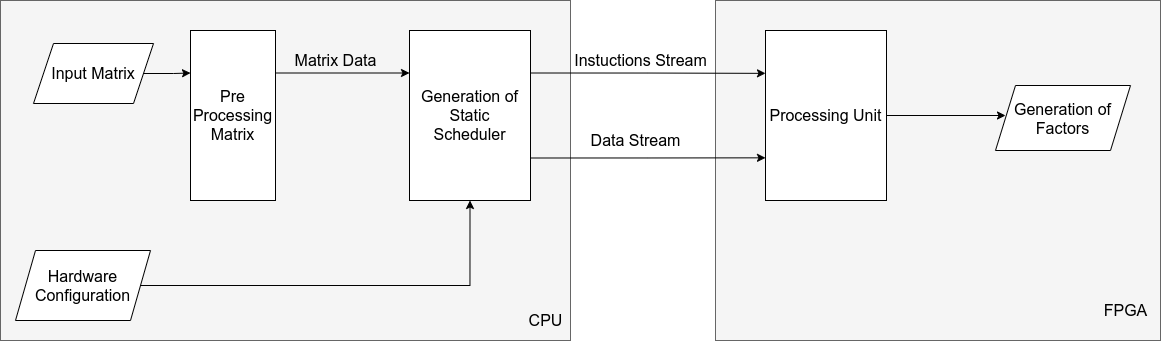
\includegraphics[width = 0.9\linewidth]{./Introduction/Introduction_flow_of_project_drawio.png}
    \caption{The overall flow of the project}
    %\label{fig:Intro:flow}
\end{figure}
\\
The summary of the thesis is given below:
\begin{itemize}
    \item Preliminaries and literature review
    \item Scheduler
    \item Hardware Design Implementation
\end{itemize} 



% \begin{figure}[h]
%     \centering
%     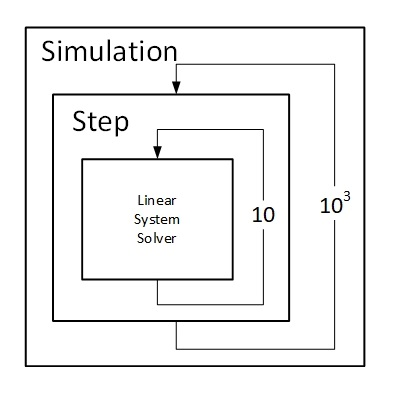
\includegraphics[width = 0.4\textwidth]{./Introduction/motive.jpg}
%     \caption{Circuit simulations typically requires several thousand solves of structurally similar linear systems}
%     \label{fig:Intro:motive}
% \end{figure}
